\documentclass{article}
\usepackage[letterpaper]{geometry}
\geometry{verbose,tmargin=1in,bmargin=1in,lmargin=1in,rmargin=1in}

\usepackage[utf8]{inputenc}
\usepackage{amsmath}
\usepackage{listings}
\usepackage{graphicx}
\usepackage{enumitem}
\usepackage{amssymb}
\usepackage{tabularx}
\usepackage{hyperref}
\usepackage{caption}
\usepackage{float}
\usepackage[section]{placeins}
\usepackage{empheq}
\usepackage{stackengine}
\usepackage{subcaption}
\usepackage{array}
\usepackage[super]{nth}

\def\delequal{\mathrel{\ensurestackMath{\stackon[1pt]{=}{\scriptstyle\Delta}}}}


\title{CIS 680: Project 2}
\author{Junfan Pan}
\date{09/27/2020}
\begin{document}
        \maketitle
    Although the solutions are entirely my own, I consulted with the following people and sources while working on this homework: \textbf{Jiatong Sun}
    \setcounter{section}{6}
    \section{Submission and Evaluation}
    \begin{enumerate}
    \item[7.1] Executing Instruction\\
    All codes are organized and executed by sequence. Simply click "Run all"and the results will show sequentially.
    \item[7.2] Data Preprocessing
    	\begin{figure}[H]
     	\centering
     	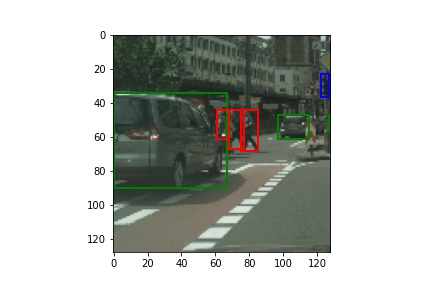
\includegraphics[width=\textwidth]
     	{images/raw_label.jpg}
     	\caption{Raw Label}
     	\label{fig:Raw Label}
     	\end{figure}
     	%\hfill
     	\begin{figure}[H]
         	\centering
         	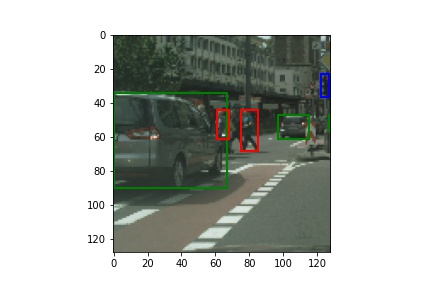
\includegraphics[width=\textwidth]
         	{images/back_label.jpg}
         	\caption{Label after converting back}
         	\label{Convert Back Label}
     	\end{figure}
      \\ 
     Comparing the images with raw labels and labels generated by converting back, we can observe that there are certain bounding box missing. The reason is that in this simplified YOLO algorithm, we only use one anchor box and its size is the same as the grid cell. Therefore, one anchor box can only identify one object instance, and if the centroids of several objects locate in the same grid cell, only one object can be detected. This explains the missing bounding box after converting back.
 
     	\begin{figure}[H]
        \centering
        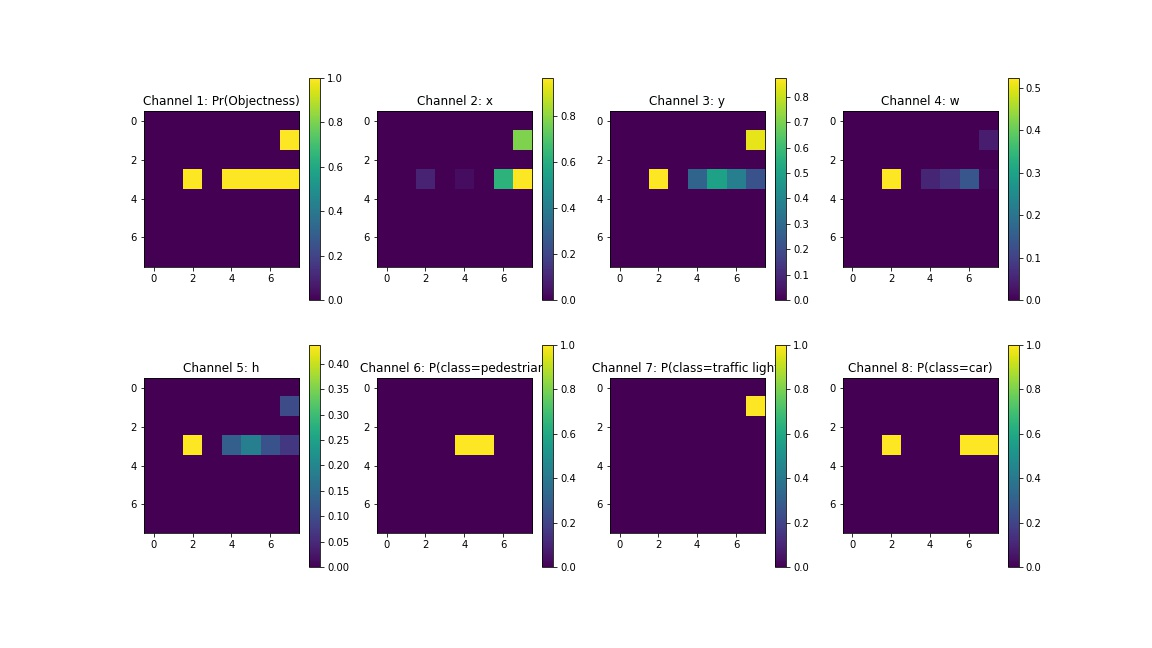
\includegraphics[width=1\textwidth]
        {images/8x8x8.jpg}
        \caption{Label of Each Channel}
        \label{fig:Label}
     	\end{figure}

     \item[7.3] Model Architecture
     \begin{figure}[H]
     	\centering
     	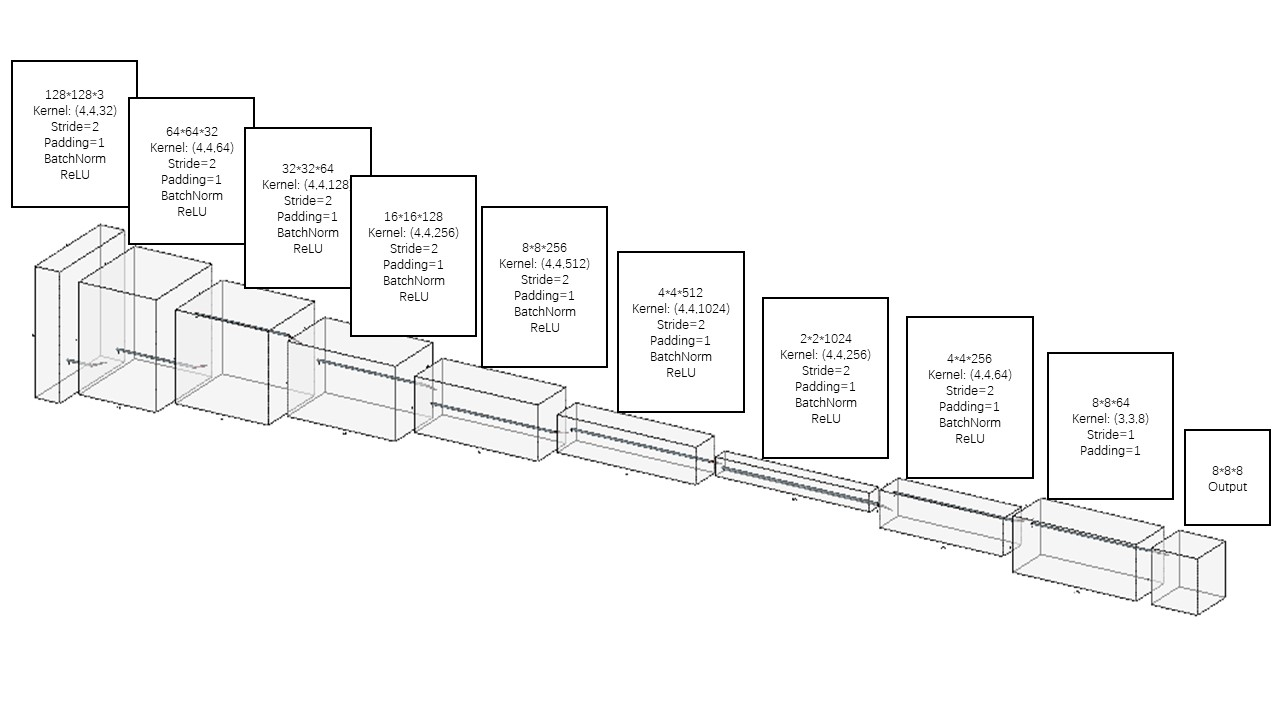
\includegraphics[width=1.15\textwidth]
     	{images/new block.jpg}
     	\caption{Model Architecture}
     \label{fig:Model Architecture}
     \end{figure}
 There is no deviation I made from the described architecture.
     \item[7.4] Training Loss
     \begin{figure}[H]
     	\centering
     	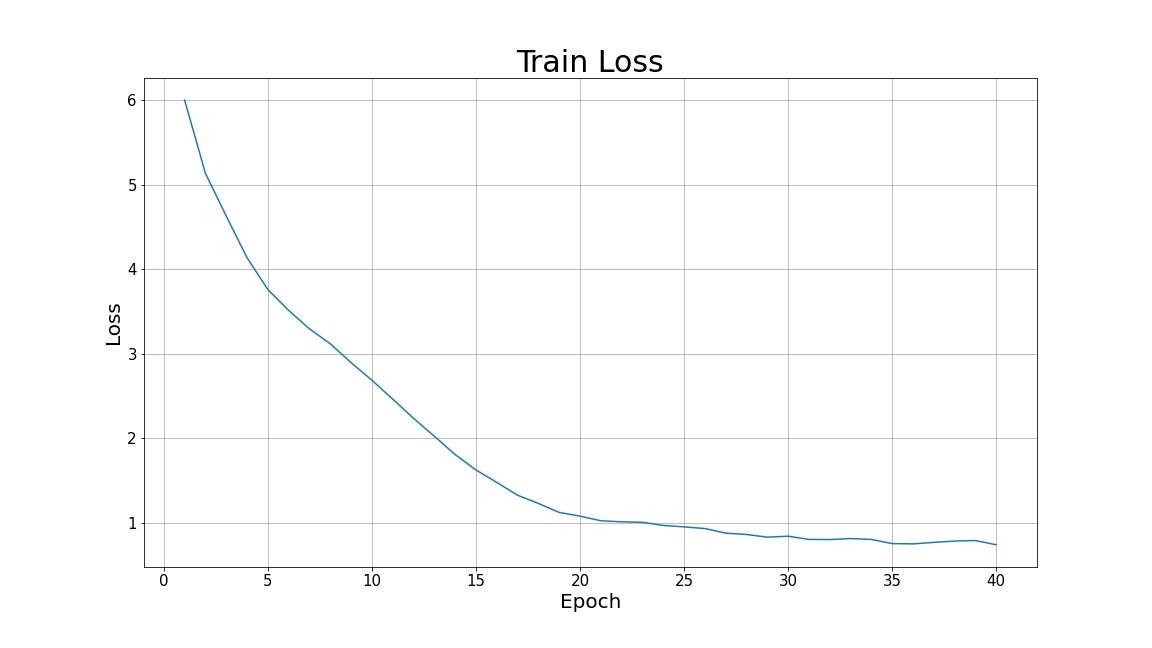
\includegraphics[width=0.7\textwidth]
     	{images/train_loss.jpg}
     	\caption{Training Loss}
     \label{fig:Training Loss}
     \end{figure}

    \end{enumerate}
    
        
\end{document}  

